\section{Legislación.}

El conjunto de los principales países desarrollados del mundo están cada vez más concienciados acerca del impacto medioambiental que tiene el actual desarrollo de la sociedad de consumo y por ello están surgiendo cada vez más iniciativas legislativas tratando de desarrollar un marco legal que permita continuar con el desarrollo de esta sociedad pero minimizando el impacto medio ambiental. A continuación haremos un pequeño repaso de las diferentes iniciativas legislativas surgidas en el ámbito de la Unión Europea, los Estados Unidos de América y Japón, como máximos representantes de los países desarrollados e industrializados.

\subsection{Naciones Unidas.}

Las Naciones Unidas ya ha mostrado su preocupación por la evolución del volumen de desechos electrónicos y por el impacto que tienen los mismos en el medio ambiente. En Julio de 2009 publicó un informe titulado, \emph{Reciclaje, de la E-basura a recursos. \cite{onu-e-waste}} donde se analizaba la evolución de la industria del reciclaje de dispositivos electrónicos en varios países en vías de desarrollo, entre ellos Sudáfrica, India y China. El objetivo final del informe era establecer las bases para la elección de los lugares donde se podría desarrollar un centro de innovación y excelencia en reciclaje de dispositivos electrónicos. 

\subsection{Unión Europea.}

La Unión Europea es uno de los principales legisladores en materia de reciclaje y reutilización de componentes electrónicos. Según palabras del comisario de medio ambiento Stavros Dimas:

\begin{quote}

\small Como la sociedad actual esta incrementando su dependencia del equipamiento eléctrico y electrónico, es muy importante que estos tengan el impacto más pequeño posible en el medio ambiente.

\end{quote}

En Agosto 2004 aprobó varias directivas que restringían el uso de sustancias potencialmente perjudiciales para la salud y para el medio ambiente en los dispositivos eléctricos y electrónicos y promovía la recogida y reciclaje de estos dispositivos una vez que no fueran necesarios. Transcurridos más de 4 años, sólo un tercio de estos dispositivos eran tratados según los protocolos establecidos por estas directivas. Aproximadamente 2,5 millones de toneladas en 2005 fueron recicladas de unos 10 millones de toneladas de residuos electrónicos. Muchos de los dispositivos están siendo tratados o depositados en vertederos fuera de la Unión Europea donde la legislación es mucho más laxa.

Por todo esto, en Julio 2012, se ha publicado la nueva directiva WEEE \cite{WEEE}. Esta nueva directiva establece un objetivo de reciclaje del 65\% de toda la basura eléctrica y electrónica y objetivos superiores para países con alto consumo de dispositivos de esta naturaleza. Además, esta directiva, apuesta por incrementar los objetivos de reutilización, dado que proporcionan un mayor valor económico y social, en línea con la línea argumental propuesta en \cite{reusing-silicon}.

\subsection{Estados Unidos de América.}

Actualmente no existe legislación federal (aplicable a todos los estados) para el reciclaje de la e-basura. Ha habido numerosos intentos para desarrollar una ley federal pero hasta la fecha no ha sido posible conseguir un consenso entre todos los estados.

No obstante, muchos de los estados, han generado políticas de reciclaje. A continuación se muestra un mapa de los Estados Unidos de América \cite{ercc}, donde se pueden ver en color azul, los diferentes estados que han legislado a favor del reciclaje de la e-basura:

\begin{figure}[H]
\begin{center}
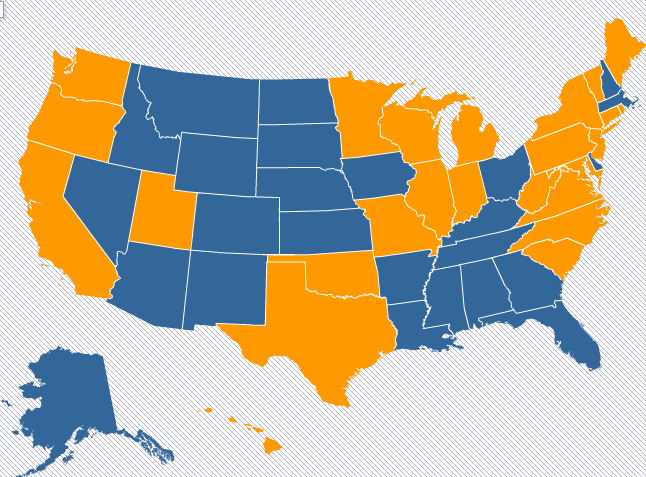
\includegraphics[width=0.8\textwidth]{img/usa_map}
\caption{Mapa de los estados con leyes aprobadas para el reciclaje y reutilización de la basura electrónica.}
\end{center}
\end{figure}

Las estadísticas de reciclaje y reutilización \cite{epa-statistics} son bastante similares a las ya comentadas de la Unión Europea. En el año 2009 un 38\% de los ordenadores era recogido para su reciclaje, un 17\% de las televisiones y tan solo un 8\% de los dispositivos móviles.

\subsection{Japón.}

Japón puede considerarse el pionero del tratamiento de los residuos electrónicos. Es comprensible, que dados los problemas generados por sus limitaciones de tamaño, debe realizar un tratamiento inteligente de los residuos para minimizar el espacio que ocupa con los mismos. En 1970, comenzó a tratar estos residuos de forma diferencial, contrataron y entrenaron a trabajadores específicamente para desmantelar y reciclar toda la e-basura, que en esas fechas, todavía no era conocido bajo este nombre. El alto coste económico de este programa llevo a Japón a abandonarlo y aplicar políticas similares a las del resto del mundo.

No obstante, en el año 2000 volvió a legislar en beneficio del reciclaje y de la reutilización de los componentes de los dispositivos electrónicos. En concreto, promulgo la ley \emph{Lay for promotion of effective utilization of resources \cite{LPEUR}} . En esta ley, en los objetivos de la misma, se menciona:

\begin{itemize}

\item{Japón necesita importar la mayor parte de los recursos básicos.}

\item{Con el desarrollo de la economía Japonesa y de su sociedad, un ingente número de dispositivos ha sido utilizado y finalmente descartado por los consumidores para seguir siendo usado.}

\item{Todos estos dispositivos descartados contienen gran cantidad de recursos y partes reutilizables que actualmente no están siendo aprovechadas.}

\item{Las medidas de la ley buscan promover el reciclaje y la reutilización de estos recursos y estas partes como motor del desarrollo de la economía del país}.

\end{itemize}

En concreto la ley prevé unos impuestos y tasas que los consumidores deben pagar en concepto de distribución y reciclaje de los dispositivos que adquieren. También prevé que las empresas deben encargarse por ley del reciclaje y de la reutilización de los dispositivos que venden. Los ingresos de estas nuevas tasas permitieron a las compañías japonesas invertir en el desarrollo de plantas de reciclaje y reutilización. 

Esto ha conseguido elevar los niveles de reciclaje por encima de los comentados de la Unión Europea y los Estados Unidos. Por ejemplo, el porcentaje de reciclaje de aires acondicionados y de televisiones esta cercano al 80\% \cite{japan-report}.

\subsection{Conclusiones.}

En resumen, los principales países desarrollados están tratando de legislar y de poner en marcha iniciativas para la disminución del volumen y del impacto de la e-basura. No obstante, estas medidas están lejos todavía de obtener unos resultados ampliamente satisfactorios. Buena parte de la legislación sólo promueve mejores prácticas y recomendaciones sin obligar a las propias naciones, compañías, instituciones y consumidores a adoptar una actitud responsable en este ámbito.